\chapter{Research Methodology} 
This chapter presents the implementation process of the research study. It explains how ClassiFish: A Mobile Application for Fish Classification and Species Information Using YOLOv11 with User Feedback Reporting was developed using the CRISP-DM and SDLC frameworks. Figure 4.1 below illustrates the Research Design Workflow of the methodology used in this study.

\begin{figure}[H]
    \centering
    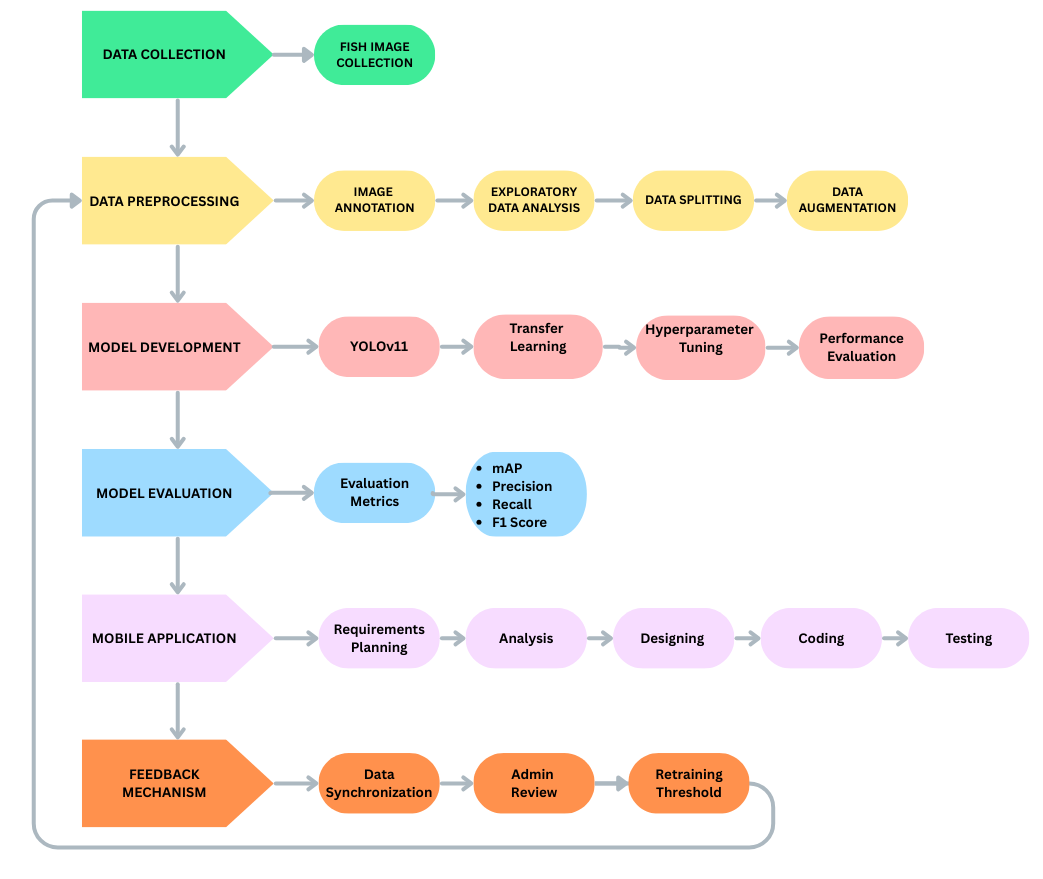
\includegraphics[width=14cm,height=10cm]{images/images/workflow.png}
    \caption{Research Design Workflow} 
\end{figure}

\noindent\large\textbf{Research Design} \newline
The development in this study is guided by two frameworks. For model development, the study follows the \textbf{CRISP-DM (Cross-Industry Standard Process for Data Mining)} framework, which consists of phases: 

\begin{itemize}
 \item\textbf{First phase: Business understanding}: Identifies the objectives of the study and how a detection model can address a practical classification need.
 \item\textbf{Second phase, Data Understanding}: Involves gathering relevant image data and examining its quality and characteristics.
 \item\textbf{Third phase, Data Preparation}: Focuses on cleaning, labeling, and organizing the image dataset for training.
 \item\textbf{Fourth phase, Modeling}: Involves applying an object detection algorithm and tuning it to achieve reliable classification results.
 \item\textbf{Fifth phase, Evaluation}: Evaluates the performance of the model to ensure it meets the intended objectives.
 \item\textbf{Sixth phase, Deployment}: Integrates the trained model into a usable application.
\end{itemize}

The Figure 4.2 below shows the CRISP-DM (Cross-Industry Standard Process for Data Mining) phases diagram, outlining each stage of the process.

\begin{figure}[H]
    \centering
    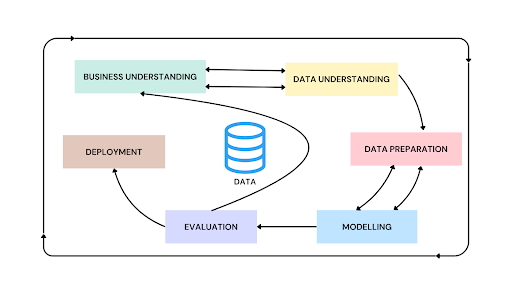
\includegraphics[width=0.8\textwidth, height=0.7\textheight, keepaspectratio]{images/images/CRISP_DM.png}
    \caption{CRISP-DM (Cross-Industry Standard Process for Data Mining)}
\end{figure}



\noindent\textbf{Software Development Life Cycle (SDLC)}\newline
For mobile application development, the study employs the Software Development Life Cycle (SDLC) framework. It guides the process from the initial concept to the implementation and maintenance, ensuring a functional and user-friendly mobile system that supports the capabilities of the model. The phases in the SDLC are:

\begin{itemize}
    \item\textbf{First phase, Planning}: Defines the scope, objectives and resource requirements of the project.
    \item\textbf{Second phase, Analysis}: Involves gathering and reviewing requirements to understand what the system must achieve.
    \item\textbf{Third phase, Design}: Focuses on creating the system architecture, interface layouts, and technical specifications.
    \item\textbf{Fourth phase, Implementation}: Involves writing and integrating the code based on the design plans.
    \item\textbf{Fifth phase, Testing}: Ensures that the system functions correctly and meets the specified requirements.
    \item\textbf{Sixth phase, Deployment}: Releases the system for actual use in its intended environment.
    \item\textbf{Seventh phase, Maintenance}: Includes monitoring, updating and fixing problems.
\end{itemize}

\noindent\textbf{Business Understanding}:\newline
As the first phase of CRISP-DM, it involved identifying a gap in existing fish species identification methods, which primarily focused on species recognition. To address this, the study aimed to develop a system that not only detected fish species but also provided nutritional and ecological information, along with a user feedback mechanism. This made the system a valuable tool for environmentalists, researchers, and consumers.

\section{Data Collection}
Data collection is part of the \textbf{Data Understanding Phase}, the second stage in the CRISP-DM framework. This phase involves gathering and exploring relevant data to guide the preparation and modeling stages.

\noindent The fish images that will be used in this study will be collected from various local wet markets in Iligan City. The fish species to be photographed will already be deceased and displayed on the vendor's stall, having been taken out of the water prior to image capture. A smartphone's rear camera will be used to photograph the entire body of the fish under natural lighting, capturing images from different angles and distances. A total of 150 raw images will be obtained for each of the 18 fish species, resulting in a dataset of 2,700 raw fish images.


\section{Data Preprocessing}
Data preprocessing is part of the \textbf{Data Preparation Phase}, the third stage in the CRISP-DM framework. This phase focuses on organizing and cleaning the data to ensure it is suitable for modeling. This section outlines the processes involved in preparing and refining the dataset for the development and training of the YOLOv11-based fish species classification model.

\subsection{Image Annotation}
For annotating the fish species image dataset, the captured fish species images will be stored on Google Drive and then imported into Label Studio for annotation. Each fish image will be manually annotated by drawing bounding boxes around the entire body of the fish for object detection. The annotation process will be needed to label the object of interest, specifying their type to train computer vision models. 

\subsection{Exploratory Data Analysis}
In preparing the annotated images for training the model, an exploratory data analysis will be undertaken to enhance the dataset's quality and consistency. This process will involve assessing the data quality, such as removing image duplicates and corrupt images that can introduce bias and hinder the model's ability to generalize, as well as visualizing the fish species dataset.

\begin{itemize}
  \item \textbf{Removing Duplicates:} To identify and eliminate duplicate entries to prevent redundancy and biased training.
  \item \textbf{Handling Corrupted Images:} To detect and address corrupted files, such as images that are unreadable.
  \item \textbf{Visualization Diagram:} To check the consistency and distribution of images across all 18 fish species and to help identify any imbalances and anomalies in the dataset.
\end{itemize}


\subsection{Data Splitting}
To facilitate the training and evaluation of the fish species classification model, the fish species image dataset containing 2,700 raw images will be partitioned into 70\% training, 15\% validation, and 15\% testing subsets. The dataset will be split by randomizing the images to ensure an even distribution of all fish species across the subsets.

\subsection{Data Augmentation}
To enhance the dataset's robustness and the classification model's generalization capability, data augmentation will be applied to the training dataset. This study will utilize a 4x augmentation technique on the dataset to improve the model’s generalization ability such as  Contrast Limited Adaptive Histogram Equalization (CLAHE), Horizontal flipping, Vertical flipping, and  Hue saturation.



\section{Model Development}
Model development is part of the \textbf{Modeling Phase}, the fourth stage in the CRISP-DM framework. This phase focuses on training and optimizing the YOLOv11 model through procedures such as hyperparameter tuning and validation.


\subsection{Model Training}
The model will be trained to recognize and classify 18 different fish species. The model will learn to predict the correct class label for each fish, as well as its location within the image, using bounding box coordinates. The images will undergo data preprocessing. During training, the model will be fed batches of annotated images to learn the visual patterns associated with different fish species. The model will be trained using a supervised learning approach, where it will compare its predictions to the true labels (species names) and adjust its internal parameters accordingly to minimize errors.

\subsection{Transfer Learning}
To enhance the training process, the model will leverage transfer learning. YOLOv11 will be initialized with pre-trained weights from models that were trained on large, diverse datasets such as Common Objects in Context (COCO). This allows the model to start with a set of learned features, particularly for object detection, and fine-tune these weights on the specific task of fish species detection.

\subsection{Hyperparameter Tuning}
Hyperparameter tuning is a critical step in optimizing the performance of the YOLOv11 model. This involves adjusting various training parameters that directly affect the learning process. Key hyperparameters include the \textbf{learning rate,}, which controls how quickly the model updates its weights; the \textbf{batch size}, which determines how many samples are processed at once; and \textbf{number of epochs}, indicating how many times the model passes over the entire dataset. Each of these parameters plays a significant role in determining how effectively the model learns from the training data.

\subsection{Performance Evaluation}
To evaluate the trained model's effectiveness and its ability to generalize to new data, validation was performed after the completion of the full training process. An independent validation dataset, different from the training data, was used to evaluate the model's performance. This post-training evaluation provided insights into the model's overall accuracy and helped identify potential issues such as overfitting.


\section{Model Evaluation}
Model evaluation is part of the \textbf{Evaluation Phase}, the fifth stage in the CRISP-DM framework. This phase focuses on assessing the model’s performance. During and after training, the model’s performance will be evaluated using several key metrics to ensure that it meets the desired efficiency levels. These metrics include:


\begin{itemize}
\item \textbf{mAP (mean Average Precision):} This will be the primary metric for assessing the model’s overall performance, providing an indication of its ability to correctly detect and classify fish species across all classes.
\item \textbf{Precision:} The ratio of correctly predicted positive fish species to the total predicted positive instances.
\item \textbf{Recall:} The ratio of correctly predicted positive fish species to all actual positive instances.
\item \textbf{F1 Score:} The harmonic mean of precision and recall, providing a balanced metric that takes both false positives and false negatives into account.
\end{itemize}

For the evaluation of the model, it will use mAP (mean Average Precision). It is a common metric for object detection models. It is also calculated as the mean Average Precision (AP) scores for all the classes in the dataset (Hui, 2018). The following evaluation tools will also be used for the evaluation of the model performance; Precision, Recall, and F1. True Positive is when the model correctly predicts the positive class. True Negative is when the model correctly predicts the negative class. False Positive is when the model incorrectly predicts the positive class and lastly False Negative is when the model incorrectly predicts the Negative Class.
\begin{center}
    \textbf{TP} = True Positive \\
    \textbf{TN} = True Negative \\
    \textbf{FP} = False Positive \\
    \textbf{FN} = False Negative
\end{center}

\noindent Precision is the ratio of true positives to all positives detection. It gives us the result of how many objects were correctly predicted. A high precision suggests that the model has low false positives. It is given in the equation. \\

\begin{equation}
\text{Precision} = \frac{\text{True Positive (TP)}}{\text{True Positive (TP)} + \text{False Positive (FP)}}
\end{equation}\\

\noindent Recall is the ratio between true positives to all positive instances. This evaluates to how well the model captures and predicts the object including those that were not predicted. Is is given in the equation\\

\begin{equation}
\text{Recall} = \frac{\text{True Positive (TP)}}{\text{True Positive (TP)} + \text{False Negative (FN)}}
\end{equation}\\

\noindent F1 is the ratio between Precision and Recall. It is to provide an evaluation when both false positives and false negatives are significant. It is given in the equation.
\begin{equation}
F_1 = 2 \cdot \frac{\text{Precision} \cdot \text{Recall}}{\text{Precision} + \text{Recall}}
\end{equation}\\


\section{Mobile Application Development}
Mobile application development primarily follows the Agile Software Development Life Cycle (SDLC) approach, organized into sprints to ensure iterative progress with continuous user feedback. While the development process is guided by SDLC, it also aligns with the \textbf{Deployment Phase}, the sixth stage of the CRISP-DM framework, since the trained model is deployed within the mobile application for end-user use.

\subsection{Requirements Collection and Planning}
\begin{itemize}

 \item \textbf{Initial Requirements:} Identify requirements based on study objectives, system functionality, and technical considerations. The focus will be on integrating YOLOv11 in the mobile application, displaying fish species information, and implementing feedback mechanisms.
 
 \item \textbf{Product Backlogs:} Convert the initial requirements into product backlogs, which will be updated throughout the development sprints. 
 
 \item \textbf{Sprint Planning:} At the start of each sprint, a meeting will be held to select items from the backlog, break them down into tasks, and define sprint goals. Each sprint focuses on a specific feature (e.g., model integration, UI/UX design, etc.).
 
 \item \textbf{Ecological and Nutritional Information:} Ecological and nutritional information will be sourced from reputable databases, websites, or studies related to marine biology and fish species. Potential sources include government fisheries websites, academic publications, and research organizations.
\end{itemize}

\subsection{Analysis}
\begin{itemize}
    \item \textbf{Technical Feasibility Assessment:}
    Evaluate the technical feasibility of integrating YOLOv11 within the mobile application. This evaluation will involve assessing the model’s performance on mobile devices and ensuring that the overall user experience remains smooth and responsive.

     \item \textbf{Key Mobile Application Features:} 
    Identify the main features from the user's perspective. These include capturing images through the camera or selecting from the gallery, detecting fish species, displaying ecological and nutritional information, and enabling feedback submission.
\end{itemize}

\subsection{Coding}
\begin{itemize}
 \item \textbf{Mobile App Development (Sprint 1-2):} Develop the mobile app using the Flutter framework. This will allow the app to work on both Android and iOS platforms. The app will integrate the camera plugin to capture fish images, display the predicted species, and enable feedback collection.
 \item \textbf{Server-Side Development (Sprint 2-3):} Use Django to develop the REST API and admin panel. The API will facilitate data synchronization (feedback, fish information) between the mobile app and the server. The admin panel will allow the system administrator to review feedback.
 \item \textbf{Database Implementation (Sprint 2):} Implement the SQLite database schema designed in the earlier phase, ensuring it is functional for storing and retrieving fish information, feedback, and other relevant data.
 \item \textbf{Model Integration (Sprint 3):} Convert the trained YOLOv11 model to TensorFlow Lite format and integrate it into the mobile app. This will allow the app to detect fish species from images captured by the user’s phone camera.
\end{itemize}

\subsection{Testing}
\begin{itemize}
 \item \textbf{Unit Testing:} Test individual components or features to ensure they function as expected. For example, test the camera functionality, model predictions, database queries, and API responses.
 \item \textbf{Integration Testing:} Test the integration between the mobile app, database, and API to ensure smooth communication and data synchronization.
\end{itemize}

\section{Feedback Mechanism}
The feedback mechanism also corresponds to the Evaluation and Deployment phases, the fifth and sixth stages of the CRISP-DM framework, while being an essential part of the SDLC process. This allows users to confirm the model’s predictions and provide corrections to improve system accuracy. If the prediction is incorrect, users can provide feedback by selecting the correct species from a dropdown list. The feedback data will include:

\begin{itemize}
 \item Original image.
 \item User-confirmed species.
 \item Timestamp of the feedback.
 \item Model’s initial prediction (whether correct or incorrect).
\end{itemize}

\textbf{Data Synchronization:} The feedback data will be stored locally on the device and later synchronized with the server via a RESTful API. The data will be uploaded in batches for efficiency and to minimize server load.

\textbf{Admin Review:} The feedback data will be reviewed by the system administrator through a web-based admin panel. Admins will have the ability to approve or reject feedback. Approved feedback will be used to retrain the model to improve its accuracy over time.
 
\textbf{Retraining Threshold:} A uniform threshold will be set for the number of validated incorrect classifications required across all fish species before initiating the model retraining process.For example, if the threshold is set at 100 incorrect feedback entries per species, all 18 fish species must first reach this value before retraining is manually performed. The retraining process will use the original training data split (70 percent training, 15 percent validation, 15 percent testing) to maintain consistency with the initial model performance.

\textbf{Model Deployment:} Once the model is retrained, it will be converted to TensorFlow Lite format and deployed to the mobile app. The app will periodically check the server for model updates and download the latest version in the background. Users will be notified when the app has downloaded an updated model. This ensures that the app’s fish species detection capabilities improve over time.


\noindent\textbf{System Architecture} \newline
The system architecture, shown in Figure 4.3 below, integrates hardware and software for the fish identification system. It shows how development processes focus on mobile application deployment. It includes integrating the trained model into the application and setting up a feedback mechanism.

\begin{figure}[ht]
    \centering
    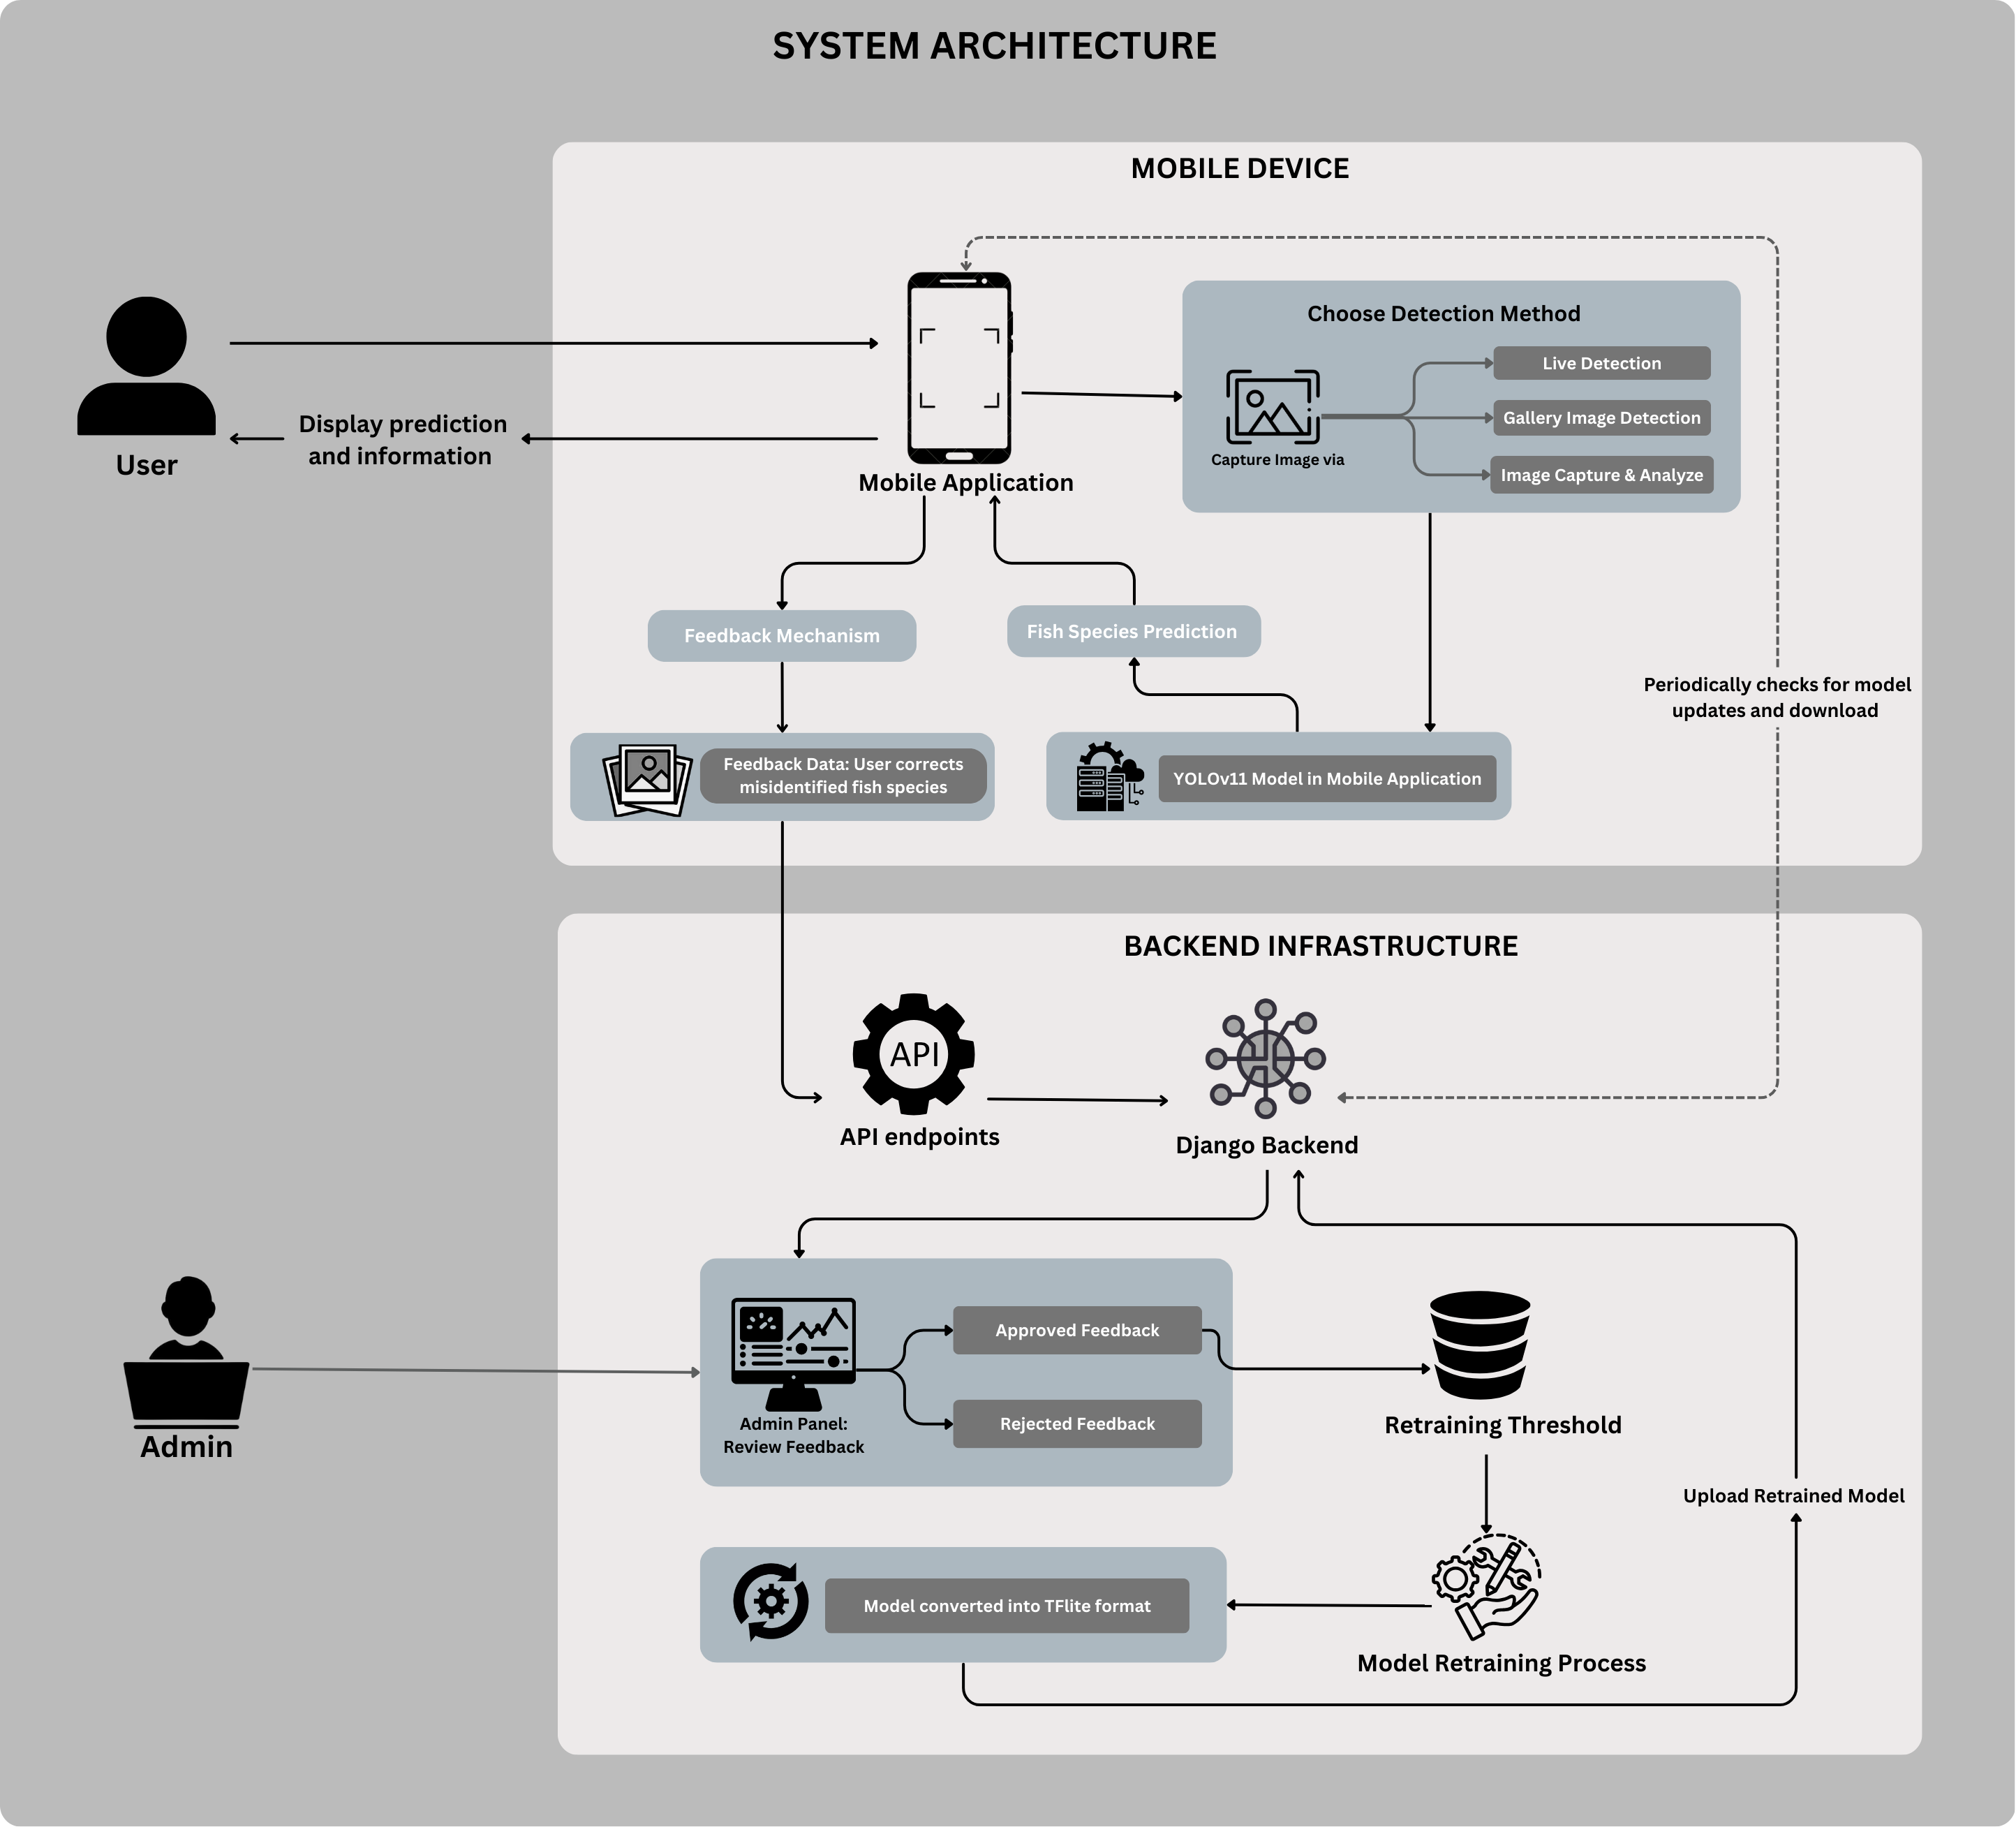
\includegraphics[width=\textwidth, height=2\textheight, keepaspectratio]{images/images/mobile_app/revision/ClassiFish_system_architecture.png}
    \caption{System Architecture}
    \label{fig:system_architecture}
\end{figure}


